\chapter{Ausarbeitung}
\section{Aufgabe 1}
Die Unsicherheit wird mit Kalmanfilter berechnet:
\begin{gather}
	\bm{P}_{n|n-1} = \bm{\Phi}_{n-1|n-1} \bm{P}_{n|n-1} \bm{\Phi}^T_{n-1|n-1} + \bm{Q} \\
	\bm{K} = \bm{P}_{n|n-1} \bm{H}_n^T \left(\bm{H}_n \bm{P}_{n|n-1} \bm{H}_n^T + \bm{R}_n \right)^{-1} \\
	\bm{P}_{n|n} = \left(\bm{I} - \bm{K}_n \bm{H}_n\right) \bm{P}_{n|n-1}
\end{gather}
Die Designmatrix $\bm{H}$ sind jeweils für 2 Fälle:
\begin{gather}
	\bm{H}_1 = 0.5 \\
	\bm{H}_2 = \cos(1 + \frac{t}{120})
\end{gather}
Die Unsicherheit von beiden Instrumenten sind in \autoref{fig:unsicherheit}.
\begin{figure}[htbp]
	\centering
	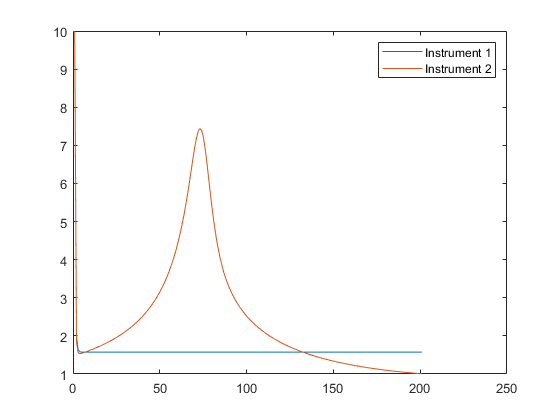
\includegraphics[width=0.7\textwidth]{images/aufgabe1} 
	\caption{Unsicherheit} 
	\label{fig:unsicherheit}
\end{figure}\\
Wenn $t \approx 70$, $p \approx \frac{\pi}{2}$ und $\cos(p) \approx 0$, der Zustand $x$ ist gegen diesem Zeitpunkt von positiv nach negativ geändert. Der Kalmanfilter braucht Zeit, um diese Änderung zu reagieren, deshalb ist die Positionsschätzung gegen $t \approx 70$ ungenauer. 
\section{Aufgabe 2}
Der Zustand wird mit Kalmanfilter jeweils vorwärts, rückwärts und kombiniert berechnet. Die Formeln für Kombination lauten:
\begin{gather}
	\bm{P}_n = \left( \left(\bm{P}^b_{n|n}\right)^{-1} + \left(\bm{P}_{n|n}\right)^{-1}\right)^{-1} \\
	\hat{\bm{x}}_n = \bm{P}_n \left( \left(\bm{P}^b_{n|n}\right)^{-1} \hat{\bm{x}}^b_{n|n} + \left(\bm{P}_{n|n}\right)^{-1} \hat{\bm{x}}_{n|n} \right)^{-1}
\end{gather}
Ergebnis:
\begin{figure}[ht]\centering
	\subfigure[$\tau_{ZWD}$]{
		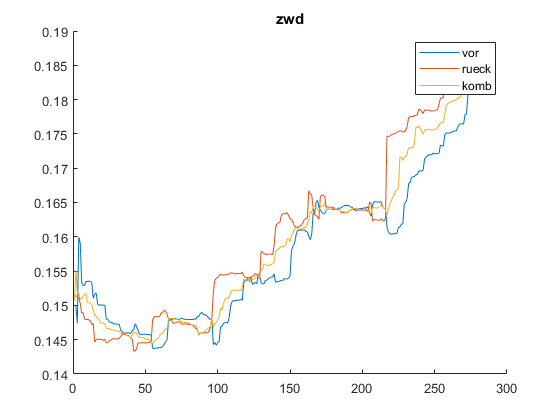
\includegraphics[width=0.45\textwidth]{zwd.png}}
	\subfigure[$\tau_{CLK}$]{
		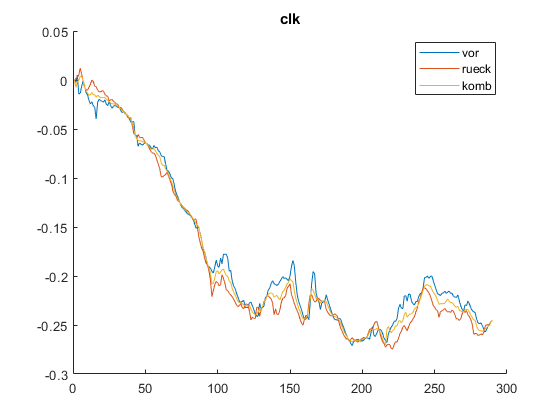
\includegraphics[width=0.45\textwidth]{clk.png}}
	\subfigure[$d \tau_{CLK}$]{
		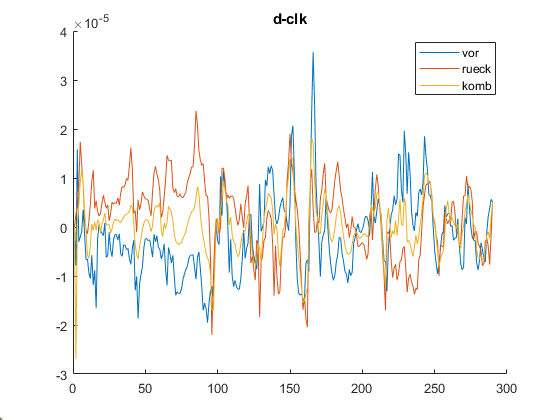
\includegraphics[width=0.45\textwidth]{dclk.png}}
	\label{fig:abstand}
\end{figure}
\clearpage
Standardabweichungen:
\begin{figure}[ht]\centering
	\subfigure[Std $\tau_{ZWD}$ vor und rückwärt]{
		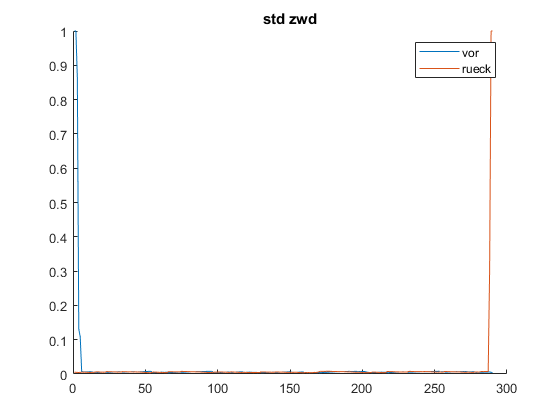
\includegraphics[width=0.4\textwidth]{stdzwd1.png}}
	\subfigure[Std $\tau_{CLK}$ kombiniert]{
		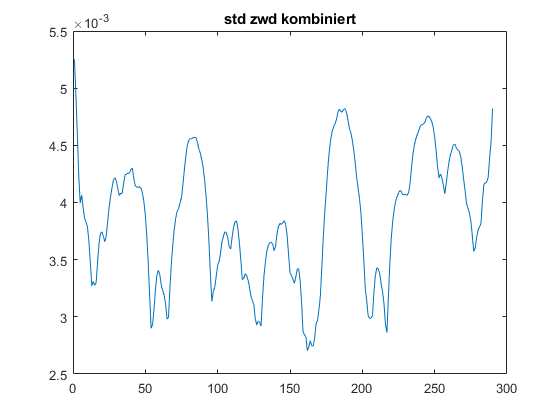
\includegraphics[width=0.4\textwidth]{stdzwd2.png}}
	\subfigure[Std $\tau_{CLK}$ vor und rückwärt]{
		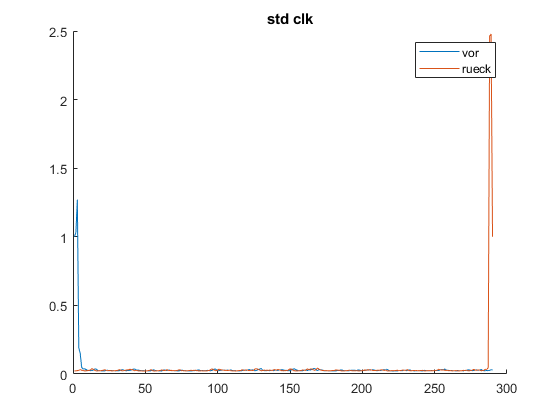
\includegraphics[width=0.4\textwidth]{stdclk1.png}}
	\subfigure[Std $\tau_{CLK}$ kombiniert]{
		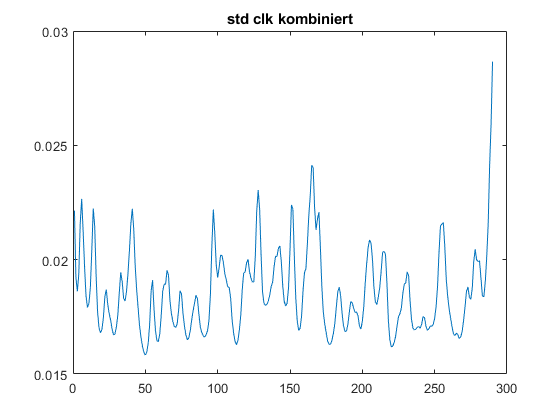
\includegraphics[width=0.4\textwidth]{stdclk2.png}}
	\subfigure[Std $d \tau_{ZWD}$ vor und rückwärt]{
		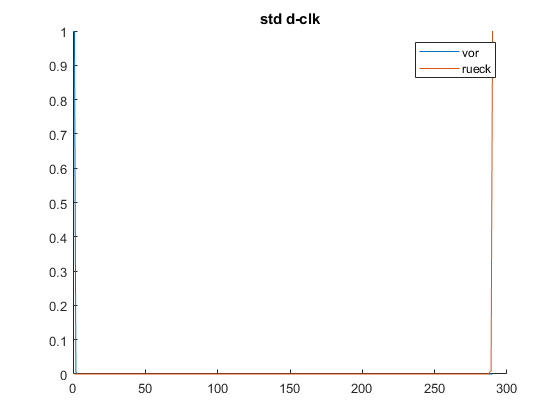
\includegraphics[width=0.4\textwidth]{stddclk1.png}}
	\subfigure[Std $d \tau_{CLK}$ kombiniert]{
		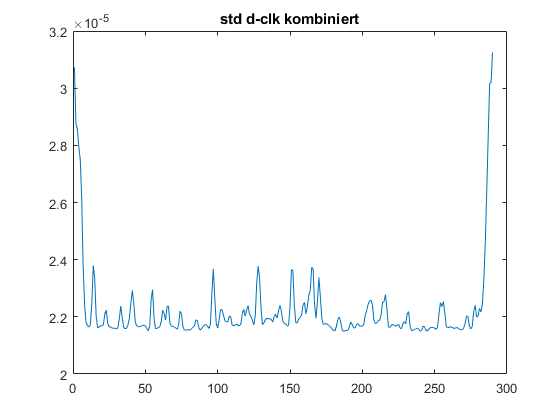
\includegraphics[width=0.4\textwidth]{stddclk2.png}}
\end{figure}